% ILLUSTRATION OF AN INTERMEDIATE ACTIVATION IN A NEURAL NETWORK
% Adapted from https://tikz.net/neural_networks/
\documentclass[tikz]{standalone}

%% PACKAGES %%
\usepackage{tikz}
\usepackage{amsmath}
\usepackage{xcolor}


%% COLORS %%
\definecolor{blue}{HTML}{0069B3}
\definecolor{lightblue}{HTML}{DCE6EB}
\definecolor{red}{HTML}{E7004A}
\definecolor{green}{HTML}{00BD67}
\definecolor{orange}{HTML}{FF9000}
\colorlet{darkblue}{blue!80!black}
\colorlet{darkgreen}{green!50!black}
\colorlet{darkred}{red!60!black}


%% CUSTOM NODES FOR TIKZ PICTURE %%
\tikzstyle{node}=[thick, circle, minimum size=22, inner sep=0.5, outer sep=0.6]
\tikzstyle{node in}=[node, blue!20!black, draw=blue!60!black, fill=blue!20!white]
\tikzstyle{node hidden}=[node, green!20!black, draw=green!60!black, fill=green!20!white]
\tikzstyle{connect}=[thick, orange, draw=blue!60!black]


\begin{document}
    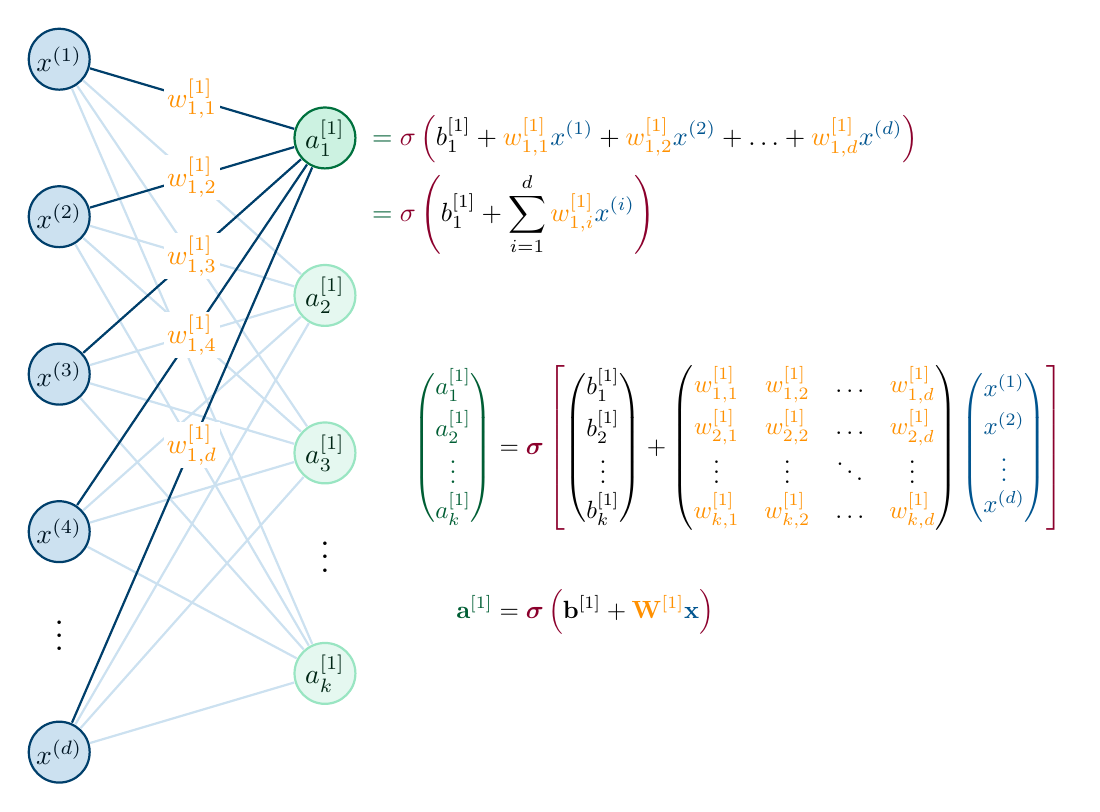
\begin{tikzpicture}[x=3.375cm, y=2cm]
      \def\NI{5}        % number of nodes in input layer
      \def\NH{4}        % number of nodes in hidden layer
      \def\yshift{0.4}  % shift last node for dots
      
      % INPUT LAYER
      \foreach \i [evaluate={\c=int(\i==\NI); \y=\NI/2-\i-\c*\yshift; \index=(\i<\NI?int(\i):"d");}]
                  in {1, ..., \NI}{  % loop over nodes
        \node[node in, outer sep=0.6] (NI-\i) at (0, \y) {$x^{(\index)}$};
      }
      
      % HIDDEN LAYER
      \foreach \i [evaluate={\c=int(\i==\NH); \y=\NH/2-\i-\c*\yshift; \index=(\i<\NH?int(\i):"k");}]
        in {\NH, ..., 1}{  % loop over nodes
        \ifnum\i=1  % single highlighted node
          \node[node hidden]
            (NO-\i) at (1, \y) {$a_{\index}^{[1]}$};
          \foreach \j [evaluate={\index=(\j<\NI?int(\j):"d");}] in {1, ..., \NI}{  % loop over nodes in previous layer
            \draw[connect] (NI-\j) -- (NO-\i)
              node[fill=white, inner sep=1pt, pos=0.50] {{$w_{1, \index}^{[1]}$} };
          }
        \else  % other light-colored nodes
          \node[node, green!20!black, draw=green!40!white, fill=green!10!white]
            (NO-\i) at (1, \y) {$a_{\index}^{[1]}$};
          \foreach \j in {1, ..., \NI}{  % loop over nodes in previous layer
            \draw[connect, blue!20!white] (NI-\j) -- (NO-\i);
          }
        \fi
      }
      
      % DOTS
      \path (NI-\NI) --++ (0, 1+\yshift) node[midway, scale=1.2] {$\vdots$};
      \path (NO-\NH) --++ (0, 1+\yshift) node[midway, scale=1.2] {$\vdots$};
      
      % EQUATIONS
      \def\arg#1{{\color{darkblue}x^{(#1)}}}
      \def\wght#1#2{{\color{orange}w_{#1, #2}^{[1]}}}
      \def\bias#1{b_{#1}^{[1]}}
      \def\actvn#1{a_{#1}^{[1]}}

      \node[below=17, right=11, darkgreen, scale=0.95] at (NO-1)
        {$\begin{aligned}
           &= \color{darkred}\sigma\left( \color{black}
                \bias{1} + \wght{1}{1}\arg{1} + \wght{1}{2}\arg{2} + \ldots + \wght{1}{d}\arg{d}
              \color{darkred}\right) \\
           &= \color{darkred}\sigma\left( \color{black}
                \bias{1} + \sum_{i=1}^{d} \wght{1}{i}\arg{i}
               \color{darkred}\right)
         \end{aligned}$};
      \node[right, scale=0.9] at (1.3, -1.3)
        {$\begin{aligned}
          {\color{darkgreen}
          \begin{pmatrix}
            \actvn{1} \\[0.3em]
            \actvn{2} \\
            \vdots    \\
            \actvn{k}
          \end{pmatrix}}
          &=
          \color{darkred}\boldsymbol{\sigma}\left[ \color{black}
          \begin{pmatrix}
            \bias{1} \\[0.3em]
            \bias{2} \\
            \vdots   \\
            \bias{k}
          \end{pmatrix}
          +
          \begin{pmatrix}
            \wght{1}{1} & \wght{1}{2} & \ldots & \wght{1}{d} \\[0.3em]
            \wght{2}{1} & \wght{2}{2} & \ldots & \wght{2}{d} \\
            \vdots      & \vdots      & \ddots & \vdots      \\
            \wght{k}{1} & \wght{k}{2} & \ldots & \wght{k}{d}
          \end{pmatrix}
          {\color{darkblue}
          \begin{pmatrix}
            \arg{1} \\[0.3em]
            \arg{2} \\
            \vdots  \\
            \arg{d}
          \end{pmatrix}}
          \color{darkred}\right]\\[2em]
          {\color{darkgreen}\mathbf{a}^{[1]}}
          &= \color{darkred}\boldsymbol{\sigma}\left( \color{black}
               \mathbf{b}^{[1]} + {\color{orange}\mathbf{W}^{[1]}} {\color{darkblue}\mathbf{x}}
             \color{darkred}\right)
        \end{aligned}$};
    \end{tikzpicture}
\end{document}
